\let\negmedspace\undefined
\let\negthickspace\undefined
\documentclass[journal]{IEEEtran}
\usepackage[a4paper, margin=10mm, onecolumn]{geometry}
%\usepackage{lmodern} % Ensure lmodern is loaded for pdflatex
\usepackage{tfrupee} % Include tfrupee package

\setlength{\headheight}{1cm} % Set the height of the header box
\setlength{\headsep}{0mm}  % Set the distance between the header box and the top of the text

\usepackage{gvv-book}
\usepackage{gvv}
\usepackage{cite}
\usepackage{amsmath,amssymb,amsfonts,amsthm}
\usepackage{algorithmic}
\usepackage{graphicx}
\usepackage{float}
\usepackage{textcomp}
\usepackage{xcolor}
\usepackage{txfonts}
\usepackage{listings}
\usepackage{enumitem}
\usepackage{mathtools}
\usepackage{gensymb}
\usepackage{comment}
\usepackage[breaklinks=true]{hyperref}
\usepackage{tkz-euclide} 
\usepackage{listings}
% \usepackage{gvv}                                        
\def\inputGnumericTable{}                                 
\usepackage[latin1]{inputenc}                                
\usepackage{color}                                            
\usepackage{array}                                            
\usepackage{longtable}                                       
\usepackage{calc}                                             
\usepackage{multirow}                                         
\usepackage{hhline}                                           
\usepackage{ifthen}                                           
\usepackage{lscape}
\usepackage{tikz}
\usetikzlibrary{patterns}

\begin{document}

\bibliographystyle{IEEEtran}
\vspace{3cm}

\title{12.76}
\author{ee25btech11063-vejith}

\maketitle
% \maketitle
% \newpage
% \bigskip
{\let\newpage\relax\maketitle}
\renewcommand{\thefigure}{\theenumi}
\renewcommand{\thetable}{\theenumi}
\setlength{\intextsep}{10pt} % Space between text and floats
\textbf{Question}\\
Four points  $\Vec{P}$ \brak{0,1}, $\Vec{Q}$ \brak{0,-3}, $\Vec{R}$ \brak{-2,-1}, $\Vec{S}$ \brak{2,-1} represent the vertices of a quadrilateral. What is  the area enclosed by the quadrilateral ?
\hfill (ST 2022)
\begin{multicols}{4}
\begin{enumerate}
\item 4
\item 4$\sqrt{2}$
\item 8
\item 8 $\sqrt{2}$
\end{enumerate}
\end{multicols}
\textbf{Solution}:\\
\begin{align}
\vec{P} = \myvec{0 \\ 1} \hspace{0.8cm}
\vec{Q} = \myvec{0 \\ -3} \hspace{0.8cm}
\vec{R} = \myvec{-2 \\ -1} \hspace{0.8cm}
\vec{S} = \myvec{2 \\ -1}
\end{align}
let PSQR be the quadrilateral then it's diagonals are $\vec{P}-\vec{Q}$ and $\vec{R}-\vec{S}$\\
\begin{align}
    \norm{\vec{P}-\vec{Q}}=\norm{\myvec{0\\4}}=4\\
    \norm{\vec{R}-\vec{S}}=\norm{\myvec{-4\\0}}=4\\
    \brak{\vec{P}-\vec{Q}}^{\top}\brak{\vec{R}-\vec{S}}=\brak{0\hspace{0.5cm} 4}\myvec{-4\\0}\\
    =0
    \end{align}
    $\implies$ diagonals of the quadrilateral are of equal length and they bisect each other perpendicularly \\
     $\implies$ the given quadrilateral is a square
     \begin{align}
         \text{area of the quadrilateral PSQR}=\frac{1}{2} \norm{\vec{P}-\vec{Q}}^2\\
         =\frac{1}{2}\times 16 =8
     \end{align}

\begin{figure}
    \centering
    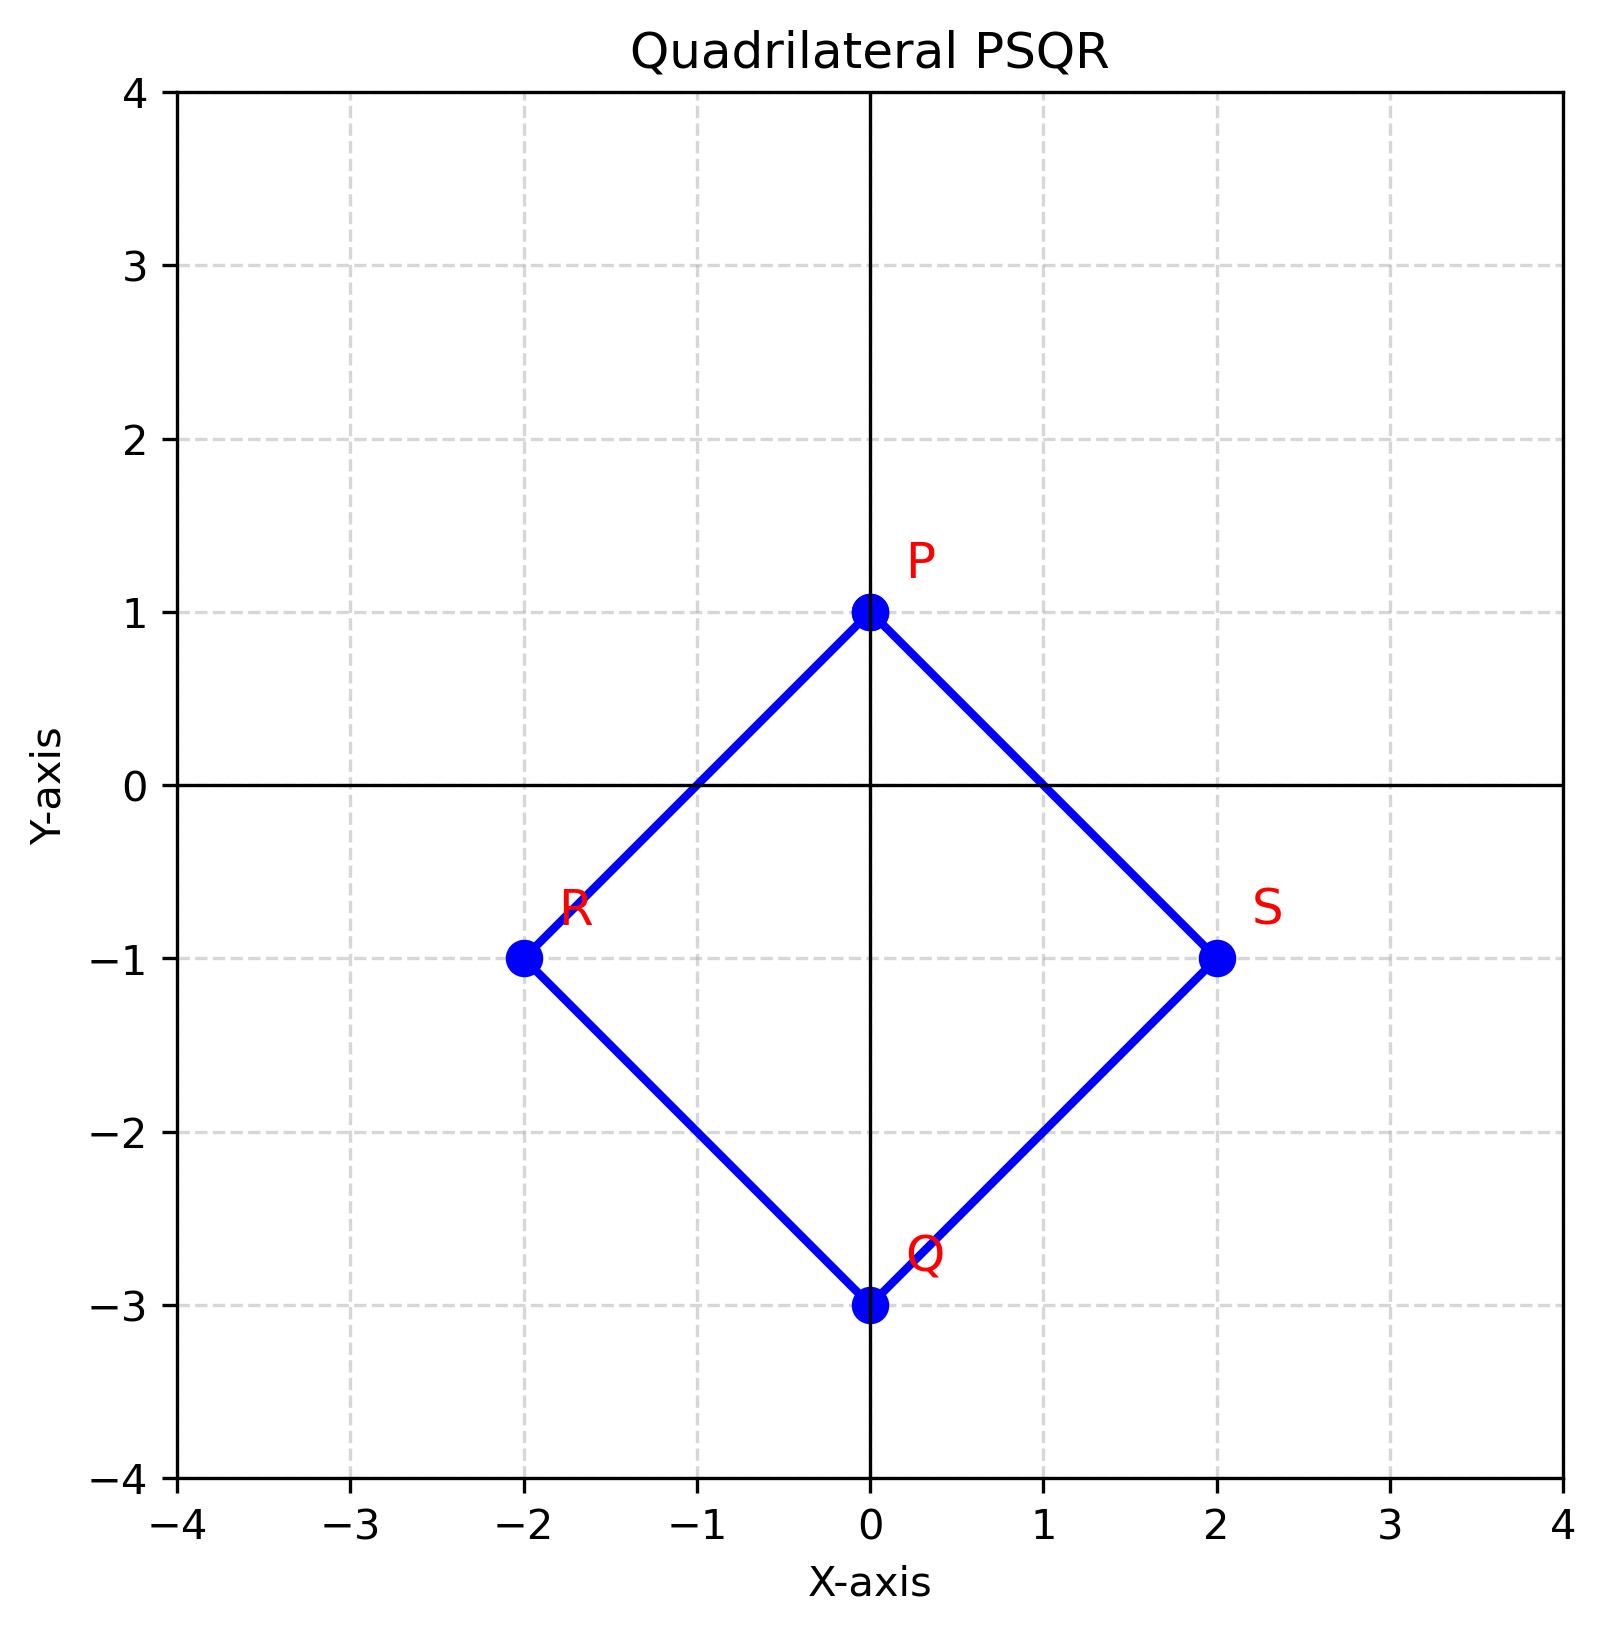
\includegraphics[width=0.52\columnwidth]{figs/01.png}
    \caption{}
    \label{fig:placeholder}
\end{figure}
\end{document}
